% !TEX root = ../main.tex
\chapter{Implementación y Arquitectura MLOps}
\label{chap:implementacion}

Este capítulo detalla la realización técnica del sistema. El proyecto se ha desarrollado como un sistema de software modular con estándares de Ingeniería de Software y MLOps: control de versiones, tipado estático, suite de tests y despliegue mediante contenedores.

\section{Arquitectura del Sistema}

El sistema se organiza en cuatro capas funcionales que transforman los datos brutos de ventas en recomendaciones de pedido operativas. La Figura~\ref{fig:arquitectura_sistema} muestra el flujo completo de datos y decisiones.

\begin{figure}[H]
\centering
\shorthandoff{>}%
\resizebox{\textwidth}{!}{%
\begin{tikzpicture}[
    every node/.style={font=\sffamily\footnotesize, align=center},
    band/.style={draw, rectangle, rounded corners=5pt,
                 minimum width=12.5cm, minimum height=1.05cm, text width=12.3cm},
    s1/.style={band, fill=blue!10},
    s2/.style={band, fill=teal!12},
    s3/.style={band, fill=orange!14},
    s4/.style={band, fill=red!10},
    s5/.style={draw, rectangle, rounded corners=5pt,
               minimum width=8cm, minimum height=0.9cm, text width=7.8cm, fill=green!14},
    mlf/.style={draw, rectangle, rounded corners=4pt, dashed,
                minimum width=2.6cm, minimum height=0.9cm, fill=gray!10},
    lbl/.style={font=\sffamily\scriptsize\bfseries, gray!75},
    arr/.style={->, thick},
    darr/.style={->, thick, dashed, gray!60}
]
  %% ── BANDAS ─────────────────────────────────────────────────────
  \node[s1] (datos)  at (0, 0)    {HF Dataset
    $\;\to\;$ Data Quality Gate (6 checks)
    $\;\to\;$ Panel Preparado};

  \node[s2] (feats)  at (0,-1.6)  {Corrección Censura (LightGBM / media histórica)
    $\;\to\;$ Feature Engineering
    $\;\to\;$ Frame Supervisado (50 features)};

  \node[s3] (model)  at (0,-3.2)  {Optuna TPE multiobj. (Pareto)
    $\;\to\;$ CatBoost Multi-Cuantil (Pinball Loss)
    $\;\to\;$ Mondrian Conformal Prediction};

  \node[s4] (dec)    at (0,-4.8)  {Newsvendor $q^*$
    $\;\to\;$ Coste de inventario
    $\;\to\;$ Nivel de servicio};

  \node[s5] (reco)   at (0,-6.2)  {\texttt{reorder\_recommendations.csv}
    $\;\to\;$ Dashboard Django};

  %% ── Registro de ejecuciones lateral ─────────────────────────────
  \node[mlf] (mlflow) at (7.8,-3.2) {\texttt{reports/}\\Registro de\\ejecuciones};

  %% ── ETIQUETAS DE CAPA ──────────────────────────────────────────
  \node[lbl, left=0.15cm of datos] {Datos};
  \node[lbl, left=0.15cm of feats] {Features};
  \node[lbl, left=0.15cm of model] {Modelado};
  \node[lbl, left=0.15cm of dec]   {Decisión};

  %% ── FLECHAS VERTICALES ─────────────────────────────────────────
  \draw[arr] (datos.south) -- (feats.north);
  \draw[arr] (feats.south) -- (model.north);
  \draw[arr] (model.south) -- (dec.north);
  \draw[arr] (dec.south)   -- (reco.north);

  %% ── Registro de ejecuciones ─────────────────────────────────────
  \draw[darr] (model.east) -- (mlflow.west);
  \draw[darr] (dec.east)   to[out=0,in=-90] (mlflow.south);

\end{tikzpicture}%
}
\shorthandon{>}%
\caption{Arquitectura del sistema: flujo de datos y decisiones entre las cuatro capas funcionales (Datos, Features, Modelado y Decisión), con persistencia de cada ejecución en un directorio versionado bajo \texttt{reports/} para trazabilidad.}
\label{fig:arquitectura_sistema}
\end{figure}

La estructura del código se organiza en torno a cuatro capas especializadas:

\begin{enumerate}
    \item \textbf{Capa de Datos}: Ingesta desde Hugging Face con un \textit{Data Quality Gate} que aborta la ejecución si detecta anomalías (datos obsoletos, duplicados o series incompletas) antes de contaminar los modelos.
    \item \textbf{Capa de Features}: Corrección de demanda censurada por stockout e ingeniería de 50 características temporales, exógenas y estáticas sin \textit{data leakage}.
    \item \textbf{Capa de Modelado}: Búsqueda Pareto de hiperparámetros (Optuna, TPE multiobjetivo), entrenamiento multi-cuantil (CatBoost con Pinball Loss) y calibración de intervalos (Mondrian Conformal Prediction).
    \item \textbf{Capa de Decisión}: Transformación de cuantiles en órdenes de pedido vía el fractil crítico del Newsvendor, y evaluación del coste de inventario y del nivel de servicio que esa política induce.
\end{enumerate}

\section{Stack Tecnológico}

La Tabla~\ref{tab:tech_stack} resume las herramientas principales del sistema. Cada elección responde a una necesidad técnica concreta, no a preferencia arbitraria.

\begin{table}[htbp]
    \centering
    \small
    \begin{tabular}{lll}
        \toprule
        \textbf{Componente} & \textbf{Herramienta} & \textbf{Alternativa descartada} \\
        \midrule
        Modelado probabilístico & CatBoost, LightGBM & XGBoost, scikit-learn \\
        Optimización multi-objetivo & Optuna (TPE multiobjetivo) & Hyperopt, GridSearch \\
        Optimización lineal & SciPy HiGHS & PuLP, CVXPY \\
        Trazabilidad de experimentos & Artefactos versionados en disco & MLflow, Weights \& Biases \\
        Capa web y API operacional & Django & FastAPI, Flask \\
        Contenerización & Docker + Compose & Entornos virtuales \\
        Validación de contratos & Pydantic v2 & dataclasses, marshmallow \\
        Explicabilidad & SHAP & LIME, eli5 \\
        Dashboard interactivo & Plantillas Django + htmx & React, Streamlit, Dash \\
        CI/CD & GitHub Actions & Jenkins, GitLab CI \\
        \bottomrule
    \end{tabular}
    \caption{Stack tecnológico del sistema con alternativas descartadas.}
    \label{tab:tech_stack}
\end{table}

Las decisiones más relevantes se justifican a continuación:

\begin{itemize}
    \item \textbf{CatBoost sobre XGBoost}: Como se argumentó en el Capítulo~\ref{chap:estado_del_arte}, CatBoost gestiona variables categóricas de alta cardinalidad (tienda, producto, categoría) de forma nativa mediante \textit{Ordered Target Statistics}, eliminando el riesgo de \textit{target leakage} que introduce el \textit{target encoding} manual en XGBoost. Adicionalmente, sus árboles oblivious actúan como regularizador implícito, beneficioso para series con alta variabilidad.

    \item \begin{sloppypar}\textbf{Optuna sobre Hyperopt o GridSearch}: Optuna implementa el sampler TPE (\textit{Tree-structured Parzen Estimator}) con soporte nativo para optimización multi\-objetivo, \textit{pruning} de trials poco prometedores y paralelización. GridSearch es inviable a escala (espacio de hiperparámetros continuo) e Hyperopt no soporta nativamente Pareto multi\-objetivo sin extensiones.\end{sloppypar}

    \item \textbf{Django sobre FastAPI o Flask}: el sistema no tiene base de datos ni servicio en línea: el estado son los artefactos que cada ejecución escribe en \texttt{reports/}, y la interfaz es un cuadro de mandos que los lee. Con ese perfil, lo que se necesita de un \textit{framework} no es asincronía sino un motor de plantillas, enrutado, sesiones y protección CSRF de serie. Django los aporta sin dependencias adicionales; FastAPI resolvía bien la superficie JSON pero obligaba a construir la capa de presentación aparte, que fue exactamente el origen de la interfaz monolítica descrita más abajo. El ORM y el sistema de migraciones quedan deliberadamente sin usar (\texttt{DATABASES} vacío), de modo que un acceso accidental a base de datos falla de forma explícita en lugar de crear un almacén silencioso.

    \item \textbf{Pydantic v2 sobre dataclasses}: Pydantic valida y convierte tipos en tiempo de ejecución, no solo en tiempo de análisis estático. Esto permite rechazar configuraciones incoherentes (ej. un horizonte negativo o una ruta de modelo inexistente) antes de que lleguen al pipeline, convirtiendo los errores tardíos en fallos rápidos y auditables.

    \item \textbf{Docker sobre entornos virtuales}: Un entorno virtual resuelve las dependencias Python pero no fija el sistema operativo, las librerías del sistema ni la versión de CUDA. Docker garantiza que el entorno de entrenamiento y el de inferencia son bitwise idénticos, eliminando la clase entera de bugs ``funciona en mi máquina''.

    \item \textbf{Renderizado en servidor sobre una \textit{Single Page Application}}: el argumento habitual para React (actualizaciones parciales de estado) no aplica aquí, porque el cliente no calculaba nada: cada movimiento de un \textit{slider} ya provocaba una llamada a la API y el servidor devolvía los números. El navegador era una capa de presentación sobre resultados ajenos. Sustituirlo por plantillas Django con htmx conserva esa actualización parcial (se intercambia solo la región de contenido) y elimina la transpilación en el navegador. La consecuencia de diseño más útil es que los parámetros del escenario pasan a vivir en la \textit{query string}: cualquier configuración del simulador es una URL compartible y recargable, algo imposible cuando el estado residía en componentes. Streamlit y Dash, que reconstruyen la página entera en cada interacción, siguen descartados por el mismo motivo que antes.
\end{itemize}

\section{Pipeline de Datos: De la Ingesta al Frame Supervisado}
\label{sec:data_pipeline}

El pipeline de datos transforma los registros de ventas crudos en el \textit{frame} supervisado que alimenta el entrenamiento del modelo. Está implementado en tres módulos especializados bajo \texttt{src/retail\_forecasting/data/} con una separación clara de responsabilidades y contratos de interfaz explícitos.

\subsection{Ingesta y Normalización (\texttt{dataset.py})}

La función \texttt{load\_raw\_split()} descarga el dataset \textit{FreshRetailNet-50K} \cite{freshretailnet2025} desde Hugging Face con caché local, seleccionando el split \texttt{train} por defecto. El resultado es un \texttt{DataFrame} con las 17 columnas brutas definidas en la especificación del dataset: siete identificadores estáticos de jerarquía (\texttt{city\_id}, \texttt{store\_id}, \texttt{management\_group\_id}, tres niveles de categoría y \texttt{product\_id}), la fecha (\texttt{dt}), las ventas brutas (\texttt{sale\_amount}) y las covariables exógenas (descuento, horas de disponibilidad, indicadores de festivo y promoción, precipitación, temperatura, humedad, viento).

La normalización construye \texttt{series\_id} concatenando \texttt{store\_id} y \texttt{product\_id}, renombra la columna de ventas a \texttt{observed\_demand} y la señal de disponibilidad horaria a \texttt{stockout\_hours}.

En esta misma etapa se descartan las filas con ventas negativas (\texttt{drop\_\allowbreak{}negative\_\allowbreak{}sales}) y las series cuyo historial es inferior a \texttt{min\_\allowbreak{}history\_\allowbreak{}days} observaciones, garantizando que cada serie tiene longitud suficiente para construir los \textit{lags}. El resultado es el \textbf{panel preparado}: una tabla indexada por (\texttt{series\_id}, \texttt{date}) sin duplicados, base para todas las etapas posteriores.

\subsection{Puerta de Calidad de Datos (\texttt{quality.py})}

Antes de iniciar ningún cálculo, el módulo \texttt{validate\_prepared\_panel()} ejecuta una batería de validaciones clasificadas en dos niveles de severidad:

\begin{itemize}
    \item \textbf{Errores bloqueantes}: La ejecución se aborta si se detectan columnas obligatorias ausentes (\texttt{date}, \texttt{series\_id}, \texttt{observed\_demand}, \texttt{stockout\_hours}), pares (\texttt{series\_id}, \texttt{date}) duplicados, nulos en columnas clave, fechas con formato inválido o datos obsoletos en modo operacional (\texttt{score\_daily}) con una antigüedad superior a \texttt{max\_}\allowbreak\texttt{data\_}\allowbreak\texttt{age\_}\allowbreak\texttt{days}.
    \item \textbf{Advertencias no bloqueantes}: Se registran en el reporte final si la fracción de valores faltantes en alguna covariable supera el umbral configurado (\texttt{max\_}\allowbreak\texttt{missing\_}\allowbreak\texttt{fraction\_}\allowbreak\texttt{warning}).
\end{itemize}

Este diseño de \textit{fail-fast} garantiza que ningún error de datos alcanza la fase de entrenamiento. Los umbrales son configurables en \texttt{DataQualityConfig} para adaptarse a distintos entornos sin modificar el código.

\subsection{Corrección de Demanda Censurada (\texttt{censorship.py})}

El módulo \texttt{LatentDemandImputer} implementa las tres estrategias de corrección descritas en la Sección~\ref{sec:demanda_censurada}: \texttt{supervised} (modelo auxiliar, estrategia por defecto), \texttt{historical\_\allowbreak{}mean} (media histórica de la serie en días sin rotura) y \texttt{clipped\_\allowbreak{}scaling} (escalado proporcional con factor configurable), más el modo \texttt{none}, que desactiva la corrección y sirve de \textit{baseline} para cuantificar el impacto de la censura. La estrategia activa es configurable en \texttt{PreprocessingConfig.}\allowbreak\texttt{imputation\_}\allowbreak\texttt{strategy}, lo que permite comparaciones controladas entre enfoques.

La estrategia \texttt{supervised} entrena un regresor LightGBM sobre las observaciones limpias (días con \texttt{stockout\_hours == 0}), usando como covariables los lags históricos de demanda, las variables de calendario y los indicadores exógenos. Después predice la demanda latente en los días censurados. El módulo añade tres columnas al panel: \texttt{latent\_}\allowbreak\texttt{demand\_}\allowbreak\texttt{est} (estimación de la demanda real), \texttt{original\_}\allowbreak\texttt{observed\_}\allowbreak\texttt{demand} (copia de las ventas originales para auditoría) e \texttt{is\_imputed} (indicador binario de las filas corregidas). El campo \texttt{observed\_demand} es sobreescrito con la estimación latente para que el pipeline de features no requiera lógica condicional. Los hiperparámetros del regresor se leen de un fichero que produce el modo \texttt{tune\_imputation}, un buscador independiente que persiste únicamente la configuración ganadora y nunca pesos ajustados, de modo que el imputador siempre reentrena sobre los días limpios del panel en curso (Anexo~\ref{anx:tuning_imputador}).

\subsection{Flujo Completo}

La Figura~\ref{fig:data_pipeline} ilustra el orden de transformaciones desde la fuente hasta el \textit{frame} supervisado listo para entrenamiento.

\begin{figure}[H]
\centering
\shorthandoff{>}%
\begin{tikzpicture}[
    node distance=0.45cm and 0.45cm,
    every node/.style={font=\sffamily\footnotesize, align=center},
    stage/.style={draw, rectangle, rounded corners=4pt, minimum width=2.5cm, minimum height=0.85cm, text width=2.3cm},
    s1/.style={stage, fill=blue!10},
    s2/.style={stage, fill=red!10},
    s3/.style={stage, fill=orange!10},
    s4/.style={stage, fill=teal!10},
    s5/.style={stage, fill=green!12},
    arr/.style={->, thick},
    modfont/.style={font=\ttfamily\tiny, gray!70}
]
\node[s1] (raw)   {Hugging Face\\FreshRetailNet-50K};
\node[s2, right=of raw]   (qgate)  {Data Quality Gate\\(6 checks)};
\node[s3, right=of qgate] (panel)  {Panel Preparado\\(series\_id, date)};
\node[s4, right=of panel] (cens)   {LatentDemand\\Imputer};
\node[s5, right=of cens]  (frame)  {Frame Supervisado\\(50 features + target)};

\draw[arr] (raw)   -- (qgate);
\draw[arr] (qgate) -- (panel);
\draw[arr] (panel) -- (cens);
\draw[arr] (cens)  -- (frame);

\node[modfont, below=0.15cm of raw]   {dataset.py};
\node[modfont, below=0.15cm of qgate] {quality.py};
\node[modfont, below=0.15cm of cens]  {censorship.py};
\node[modfont, below=0.15cm of frame] {engineering.py};
\end{tikzpicture}
\shorthandon{>}%
\caption{Pipeline de datos: flujo de transformaciones desde la ingesta hasta el frame supervisado.}
\label{fig:data_pipeline}
\end{figure}

\section{Modos de Ejecución y Ciclo Operacional}
\label{sec:run_modes}

El sistema distingue explícitamente entre operaciones de investigación y operaciones de producción mediante cuatro modos de ejecución configurables a través del parámetro \texttt{run\_mode}:

\begin{enumerate}
    \item \textbf{\texttt{experiment}}: Modo de investigación completo. Ejecuta el \textit{backtesting walk-forward} con múltiples \textit{folds} temporales, compara las estrategias de demanda observada y latente, selecciona el modelo \textit{champion} mediante \textit{promotion logic} y genera artefactos de análisis exhaustivos (\texttt{report.md}, \texttt{champion\_registry.json}, gráficos de Pareto). Es el modo utilizado para validar el sistema antes de su despliegue.

    \item \textbf{\texttt{retrain}}: Modo de refresco operacional. Entrena el modelo \textit{champion} sobre la totalidad de los datos disponibles sin realizar evaluación por \textit{folds}. Guarda el modelo en disco en formato \texttt{.pkl}. Se ejecuta periódicamente en producción para mantener el modelo actualizado con los datos más recientes.

    \item \begin{sloppypar}\textbf{\texttt{score\_daily}}: Modo de producción diario. Carga el modelo \textit{champion} guardado, construye el \textit{inference frame} con los datos más recientes y genera \texttt{reorder\_}\allowbreak\texttt{recommendations.csv}: una fila por par tienda-producto con la \texttt{order\_quantity} óptima para el horizonte $H$, los tres cuantiles calibrados (\texttt{q\_0.1},\allowbreak{} \texttt{q\_0.5},\allowbreak{} \texttt{q\_0.9}) y la fecha de decisión. Este fichero es el entregable que consumiría el sistema de compras o el responsable de reposición.\end{sloppypar}

    \item \textbf{\texttt{simulate\_ops}}: Modo de investigación MLOps. Ejecuta la simulación operacional en \textit{streaming} descrita en la Sección~\ref{sec:simulate_ops}, comparando múltiples cadencias de reentrenamiento sobre el split de evaluación.
\end{enumerate}

\subsection{Ciclo de Vida de los Hiperparámetros: Optimización vs. Reentrenamiento}
\label{sec:mlops_workflow}

Una de las decisiones críticas de diseño ha sido la separación entre la optimización estructural de los hiperparámetros y el reentrenamiento operacional diario. Siguiendo las mejores prácticas de MLOps para entornos de inventario, el sistema opera bajo un esquema de dos niveles, visualizado en la Figura~\ref{fig:mlops_flow}:

\begin{figure}[h]
    \centering
    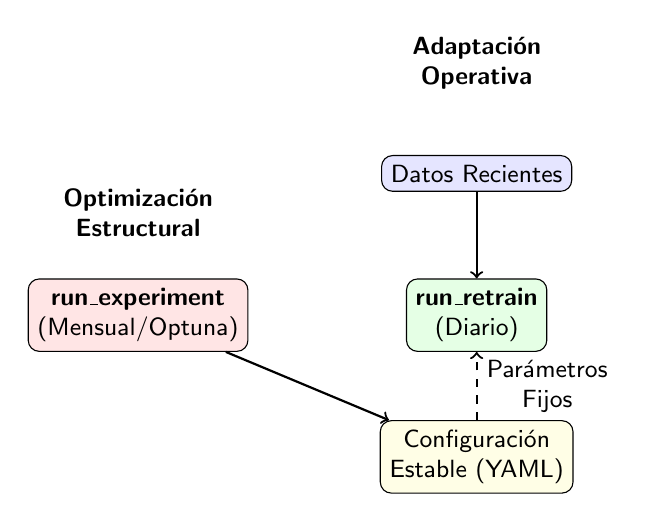
\begin{tikzpicture}[node distance=1.8cm, every node/.style={font=\sffamily\small, align=center}]
        % Nodos
        \node[draw, rectangle, rounded corners, fill=blue!10] (data) {Datos Recientes};
        \node[draw, rectangle, rounded corners, fill=green!10, below of=data] (retrain) {\textbf{run\_retrain} \\ (Diario)};
        \node[draw, rectangle, rounded corners, fill=red!10, left of=retrain, xshift=-2.5cm] (optuna) {\textbf{run\_experiment} \\ (Mensual/Optuna)};
        \node[draw, rectangle, rounded corners, fill=yellow!10, below of=retrain] (deploy) {Configuración\\Estable (YAML)};

        % Flujo
        \draw[->, thick] (data) -- (retrain);
        \draw[->, thick] (optuna) -- (deploy);
        \draw[->, thick, dashed] (deploy) -- (retrain) node[midway, right] {Parámetros\\Fijos};

        % Notas
        \node[above of=optuna, yshift=-0.5cm] {\textbf{Optimización}\\\textbf{Estructural}};
        \node[above of=data, yshift=-0.4cm] {\textbf{Adaptación}\\\textbf{Operativa}};
    \end{tikzpicture}
    \caption{Ciclo de vida MLOps: Optimización mensual vs. Reentrenamiento operativo.}
    \label{fig:mlops_flow}
\end{figure}

\begin{enumerate}
    \item \begin{sloppypar}\textbf{Fase de Optimización Mensual (Optuna)}: Ejecutado mediante el modo \texttt{experiment}, este ciclo realiza una búsqueda exhaustiva en el espacio de hiperparámetros utilizando \textit{Optuna}. Dado el volumen de datos (4.5M de filas), el sistema implementa un \textbf{muestreo estratificado por serie temporal}, limitando el entrenamiento del tuning a un máximo de 500k registros representativos. Esto garantiza que la convergencia de Optuna sea ágil sin perder la significancia estadística. Los resultados son validados mediante un análisis humano de estabilidad (comparando Pinball Loss en $q^*$ y Winkler Score), y si se identifican mejoras significativas, se actualiza el archivo \texttt{configs/\allowbreak default.yaml}.\end{sloppypar}
    \item \textbf{Fase de Reentrenamiento Operacional (Daily)}: Ejecutado mediante el modo \texttt{retrain}, este proceso es determinista y utiliza la configuración fija definida en \texttt{default.yaml}. Su función es la integración de los datos de ventas más recientes, manteniendo la lógica del modelo estable.
\end{enumerate}

Esta separación hace que el comportamiento del sistema sea predecible y auditable: si los hiperparámetros cambian cada día resulta muy difícil diagnosticar por qué una predicción fue mala. Fijar los parámetros y revisarlos con periodicidad mensual es un compromiso razonable entre adaptarse a nuevos patrones de demanda y mantener la estabilidad del sistema en producción.

\subsection{Lógica de Promoción del Modelo Campeón}
\label{sec:champion_promotion}

Al término de cada ejecución en modo \texttt{experiment}, el sistema evalúa automáticamente si algún modelo \textit{challenger} debe reemplazar al \textit{champion} actualmente registrado en \texttt{champion\_registry.json}. La decisión sigue un protocolo con dos guardarraíles configurables:

\begin{enumerate}
    \item \textbf{Mejora de coste mínima}: Se calcula la mejora relativa en coste de inventario simulado respecto al campeón actual como $\Delta_{\text{cost}} = \frac{C_{\text{champion}} - C_{\text{challenger}}}{C_{\text{champion}}} \times 100$\%. El \textit{challenger} solo es candidato si $\Delta_{\text{cost}} \geq \theta_{\text{cost}}$, donde $\theta_{\text{cost}}$ es el umbral \texttt{champion\_}\allowbreak\texttt{min\_}\allowbreak\texttt{cost\_}\allowbreak\texttt{improvement\_}\allowbreak\texttt{pct} (por defecto 0\%, modificable en \texttt{BusinessConfig}).

    \item \begin{sloppypar}\textbf{Guardarraíl de nivel de servicio}: El \textit{challenger} no debe degradar el nivel de servicio más allá de un margen configurable (\texttt{champion\_}\allowbreak\texttt{max\_}\allowbreak\texttt{service\_}\allowbreak\texttt{level\_}\allowbreak\texttt{degradation}). Si $\Delta_{\text{sl}} < -\delta_{\text{sl}}$, el candidato es descartado aunque mejore el coste.\end{sloppypar}
\end{enumerate}

Entre todos los \textit{challengers} que superan ambos guardarraíles, se selecciona el de menor coste total (con el nivel de servicio como criterio de desempate). La decisión (incluyendo los valores exactos de $\Delta_{\text{cost}}$, $\Delta_{\text{sl}}$, el motivo de aceptación o rechazo y los identificadores de ambos modelos) queda registrada en el campo \texttt{promotion} del metadato de la ejecución, garantizando una trazabilidad completa del historial de cambios de modelo. La Figura~\ref{fig:champion_promotion} muestra el flujo de decisión completo.

\begin{figure}[H]
\centering
\shorthandoff{>}%
\begin{tikzpicture}[
    node distance=0.85cm and 1.6cm,
    box/.style={rectangle, draw=gray!70, fill=gray!10, rounded corners=3pt,
                minimum width=3.8cm, minimum height=0.65cm,
                font=\sffamily\footnotesize, align=center},
    dec/.style={diamond, draw=blue!60, fill=blue!10, aspect=2.4,
                minimum width=3.8cm, minimum height=0.65cm,
                font=\sffamily\footnotesize, align=center, inner sep=1pt},
    yes/.style={font=\sffamily\scriptsize, midway, left},
    no/.style={font=\sffamily\scriptsize, midway, above},
    rej/.style={rectangle, draw=red!50, fill=red!8, rounded corners=3pt,
                minimum width=2.8cm, minimum height=0.55cm,
                font=\sffamily\footnotesize, align=center},
    ok/.style={rectangle, draw=green!50!black, fill=green!10, rounded corners=3pt,
               minimum width=3.8cm, minimum height=0.65cm,
               font=\sffamily\footnotesize, align=center}]
  % Nodes
  \node[box]  (start)  {Ejecutar \texttt{experiment}\\evaluar modelos candidatos};
  \node[dec,  below=of start]  (c1) {$\Delta_{\text{cost}} \geq \theta_{\text{cost}}$?};
  \node[dec,  below=of c1]     (c2) {$\Delta_{\text{sl}} \geq -\delta_{\text{sl}}$?};
  \node[box,  below=of c2]     (sel){Seleccionar \textit{challenger}\\de menor coste};
  \node[ok,   below=of sel]    (promo){Promover \textit{challenger}\\como nuevo campeón};
  \node[rej,  right=of c1]     (rj1){Mantener\\campeón actual};
  \node[rej,  right=of c2]     (rj2){Mantener\\campeón actual};
  % Arrows
  \draw[->,thick] (start) -- (c1);
  \draw[->,thick] (c1)    -- node[yes]{Sí} (c2);
  \draw[->,thick] (c1)    -- node[no]{No} (rj1);
  \draw[->,thick] (c2)    -- node[yes]{Sí} (sel);
  \draw[->,thick] (c2)    -- node[no]{No} (rj2);
  \draw[->,thick] (sel)   -- (promo);
\end{tikzpicture}
\shorthandon{>}%
\caption{Flujo de decisión de la \textit{promotion logic} del campeón. Un \textit{challenger}
solo reemplaza al modelo actual si supera simultáneamente el umbral de mejora de coste
($\theta_{\text{cost}}$) y el guardarraíl de nivel de servicio ($\delta_{\text{sl}}$).}
\label{fig:champion_promotion}
\end{figure}

\subsection{Trazabilidad de Experimentos}
\label{sec:experiment_tracking}

Cada ejecución escribe un directorio propio bajo \texttt{reports/}, identificado por marca temporal, que constituye el registro completo y autocontenido del experimento. Se persisten cuatro categorías de información:

\begin{itemize}
    \item \textbf{Configuración y procedencia}: \texttt{backtest\_}\allowbreak\texttt{metadata.json} recoge el dataset, las \textit{features}, la definición de los \textit{folds}, los modelos evaluados, el \textit{hash} de la configuración y el \textit{commit} de Git con el que se generó. Esos dos últimos campos son los que permiten reconstruir el experimento exacto: el \textit{hash} identifica los parámetros y el \textit{commit} el código.
    \item \textbf{Métricas}: \texttt{metrics\_}\allowbreak\texttt{summary.csv} y \texttt{cost\_}\allowbreak\texttt{summary.csv} contienen, por modelo y estrategia de datos, el coste de inventario simulado, el nivel de servicio, el Winkler Score, la cobertura condicional y el MAE.
    \item \textbf{Predicciones y decisiones}: \texttt{predictions.csv} conserva la predicción puntual, los cuantiles calibrados y la cantidad de pedido para cada par serie-fecha de validación, de modo que cualquier métrica publicada es recomputable a posteriori sin volver a entrenar.
    \item \textbf{Campeón vigente}: \texttt{champion\_}\allowbreak\texttt{registry.json} persiste entre ejecuciones qué modelo está operativo y bajo qué métricas fue promocionado, cerrando el ciclo con la \textit{promotion logic} de la Figura~\ref{fig:champion_promotion}.
\end{itemize}

Una versión anterior del sistema replicaba esta información en un servidor MLflow. Se retiró al constatar que era una segunda copia de datos que ya vivían en disco y que ninguna herramienta consumía: el cuadro de mandos lee los artefactos directamente. La trazabilidad efectiva la aportan el \textit{hash} de configuración y el \textit{commit} de Git, no el servidor; prescindir de él elimina una dependencia pesada y un contenedor sin reducir lo que puede auditarse.

\section{API REST e Interfaz Web}
\label{sec:api}

La capa web es una aplicación Django que cumple dos funciones separadas: renderiza el cuadro de mandos en servidor y expone una superficie JSON reducida para clientes máquina (sistemas de compras, \textit{scripts} de automatización). La separación es estricta: la lógica de dominio vive en \texttt{api/services/}, que no importa Django y opera sobre \textit{DataFrames}, mientras que las vistas se limitan a leer parámetros, invocar un servicio y renderizar. Esa frontera es la que permite verificar el cálculo conforme o la cantidad Newsvendor sin instanciar un cliente web.

El sistema no emplea base de datos: el estado son los artefactos en disco, y la única información propia de la capa web es la sesión del operador, transportada en una \textit{cookie} firmada.

\subsection{Superficie JSON}

Durante la migración a renderizado en servidor, los \textit{endpoints} que existían únicamente para alimentar al cliente JavaScript fueron sustituidos por vistas HTML. Se conservó el subconjunto que constituye una interfaz máquina-a-máquina real, descrito en la Tabla~\ref{tab:api_endpoints} y documentado en la propia aplicación bajo la ruta \texttt{/api/}.

\begin{table}[htbp]
    \centering
    \small
    \begin{tabular}{>{\raggedright\arraybackslash}p{3.2cm}>{\raggedright\arraybackslash}p{2.3cm}>{\raggedright\arraybackslash}p{6.5cm}}
        \toprule
        \textbf{Método + Ruta} & \textbf{Nombre} & \textbf{Descripción} \\
        \midrule
        \texttt{POST /predict\_\allowbreak orders} & Scoring operacional & Ejecuta el modo \texttt{score\_daily} y devuelve \texttt{reorder\_recommendations}: una fila por par tienda-producto con \texttt{order\_quantity}, cuantiles calibrados y fecha de decisión. \\
        \texttt{POST /api/forecast} & Simulador \textit{What-If} & Recalcula los cuantiles conformes empíricos y la cantidad óptima $q^*$ del Newsvendor dado un conjunto de parámetros (\texttt{serviceLevel}, \texttt{shortageCost}, \texttt{holdingCost}, \texttt{capacity}) y un \texttt{selectedSkuId}. \\
        \texttt{GET /api/skus} & Catálogo de SKUs & Devuelve hasta 50 SKUs con métricas calculadas sobre las predicciones del último run: cobertura empírica, PSI de drift, $q^*$ y estado operacional (\textit{ok}/\textit{drift}/\textit{shortage}/\textit{overstock}). \\
        \texttt{GET /api/\allowbreak download/\allowbreak predictions} & Descarga de predicciones & Sirve el \texttt{predictions.csv} de la ejecución más reciente, para análisis externo o auditoría. \\
        \texttt{GET /api/\allowbreak download/costs} & Descarga de costes & Sirve el resumen de costes de la ejecución más reciente. \\
        \texttt{GET /health} & Sonda de disponibilidad & Devuelve estado del servicio, versión, \textit{uptime} y si las predicciones están cargadas en caché; pensada para integrarse con herramientas de monitorización externas. Es el único endpoint público: el resto exige sesión. \\
        \bottomrule
    \end{tabular}
    \caption{Superficie JSON documentada del sistema. El monitor de drift y las alertas, que antes eran \textit{endpoints}, se sirven ahora como vistas HTML renderizadas en servidor.}
    \label{tab:api_endpoints}
\end{table}

\subsection{Cuadro de Mandos}

El cuadro de mandos se organiza en dos planos que reproducen la separación del propio sistema entre operación e investigación. El Apéndice~\ref{anexo:dashboard} recoge capturas de las siete vistas.

El \textbf{plano de Operación} responde a las dos preguntas del ciclo diario: cuánto pedir de cada SKU y qué excepciones revisar antes de aprobar el plan.

\begin{itemize}
    \item \textbf{Simulación OPS}: reproducción semana a semana del \textit{backtest} \textit{walk-forward}, con la trayectoria de una serie (predicción, banda conformal y demanda revelada) y la comparación entre cadencias de reentrenamiento.

    \item \textbf{Dashboard}: los cuatro KPIs principales (coste de inventario, cobertura empírica, MAE y PSI de \textit{drift}), el gráfico de demanda real frente a predicha con la banda conformal, y los módulos matemáticos que documentan las tres formulaciones del sistema (\textit{Conformal Prediction}, Newsvendor y optimización de capacidad).

    \item \textbf{Análisis SKU}: tabla de los SKUs activos con búsqueda, filtro por estado y ordenación, donde el gestor puede ajustar manualmente la cantidad propuesta antes de exportar el plan de reposición.

    \item \textbf{Monitor de Drift}: PSI por \textit{feature} con los histogramas de referencia y actual superpuestos, calculado por \texttt{drift/psi.py} y persistido como \texttt{drift\_report.json} al término de cada \texttt{experiment}.
\end{itemize}

El \textbf{plano de Análisis} sirve a la justificación metodológica: la vista de \textbf{EDA} publica las figuras del módulo exploratorio; \textbf{Demanda Latente} contrasta las tres estrategias de reconstrucción de censura con su veredicto de calidad; y \textbf{Pareto Tuning} muestra el frente multiobjetivo, la sensibilidad al ratio de costes y el \textit{backtest} de coste justo.

Transversal a ambos planos, el simulador \textit{What-If} permite ajustar mediante \textit{sliders} el nivel de servicio objetivo, los costes de rotura y almacenamiento y la capacidad; el servidor recalcula la política y devuelve la región de contenido actualizada. Como esos parámetros viajan en la \textit{query string}, cualquier escenario explorado queda registrado en la URL y puede compartirse o reproducirse.

Dos decisiones de implementación merecen mención por su efecto en la defensa del sistema. La primera es que \textbf{todos los gráficos se generan como SVG en el servidor}: la geometría se calcula en Python y se envía como marcado, sin librería de graficación en el cliente. La segunda es que \textbf{la ausencia de un artefacto se comunica explícitamente}: una ejecución sin \texttt{drift\_report.json} muestra un aviso que nombra el modo de ejecución que lo produce, en lugar de un panel vacío que podría confundirse con ``sin deriva detectada''.

\section{Calidad de Software e Infraestructura CI/CD}
Para garantizar que la deuda técnica no limite el escalado del sistema, se han aplicado prácticas fundamentales de \textit{DevOps}:
\begin{itemize}
    \item \textbf{Contratos Estrictos (Pydantic)}: Toda la configuración y los metadatos transitan a través de esquemas validados y tipados estáticamente, rechazando configuraciones incoherentes o derivas de datos no controladas.
    \item \textbf{Contenerización (Docker)}: La aplicación Django, que sirve tanto el cuadro
    de mandos como la superficie JSON, se despliega sobre un servidor ASGI y se orquesta junto
    a un proxy inverso Caddy mediante \texttt{docker-compose.yml}, garantizando que cualquier
    investigador pueda levantar la arquitectura completa con un solo comando en cualquier
    sistema operativo.
    \item \textbf{Integración Continua (GitHub Actions)}: El repositorio cuenta con un pipeline de CI (\texttt{ci.yml}) que, ante cada nuevo \textit{commit}, despliega un entorno virgen, verifica el estilo y el formato del código (Ruff), comprueba los tipos estáticos (Mypy) y ejecuta la batería de tests automatizados descritos en la sección siguiente.
\end{itemize}

\subsection{Estrategia de Testing: Pirámide de Verificación}
\label{sec:testing}

El sistema cuenta con 20 módulos de test organizados en cinco niveles, cada uno orientado a un tipo de fallo diferente (Tabla~\ref{tab:test_strategy}).

\begin{table}[htbp]
    \centering
    \small
    \begin{tabular}{lp{9.5cm}}
        \toprule
        \textbf{Nivel} & \textbf{Qué verifica} \\
        \midrule
        Contratos de datos & Esquemas, tipos y rangos de los DataFrames producidos por cada etapa. \\
        Anti-\textit{data leakage} & Que ninguna feature contiene información del periodo de predicción. \\
        Contratos de configuración & Que los guardarraíles experimentales se preservan ante cambios de config; correctitud aritmética de Pinball Loss por cuantil. \\
        Unitarios de lógica & Correctitud aritmética de lags, Winkler Score y Newsvendor. \\
        Integración y humo & Pipeline end-to-end sobre datos sintéticos, vistas y \textit{endpoints} de la capa web, y CI/CD. \\
        \bottomrule
    \end{tabular}
    \caption{Estrategia de testing por niveles: 20 módulos clasificados por tipo de fallo.}
    \label{tab:test_strategy}
\end{table}

El nivel más crítico es el de los \textbf{tests anti-\textit{data leakage}}, poco habitual en proyectos de ML pero imprescindible aquí: verifican que ningún lag usa el valor del propio día de predicción, que las covariables realizadas (descuento, stockout, clima) solo entran al modelo como pasado, y que el backtesting walk-forward respeta el gap de $H$ días entre el último día de entrenamiento y el primero de test. Estos tests se ejecutan automáticamente en el pipeline de CI antes de cada \textit{merge}.

\section{Explicabilidad y Diagnóstico Automático}
Un sistema de apoyo a la decisión en \textit{retail} pierde su valor si opera como una caja negra. Por ello, se han integrado módulos de observabilidad (\textit{Observability}):
\begin{itemize}
    \item \textbf{Explicabilidad Global (SHAP)}: El sistema genera valores de Shapley Aditivos \cite{lundberg2017shap} (\texttt{shap}) para el modelo Campeón, documentando gráficamente el peso real de los \textit{lags}, las variables climáticas o las jerarquías en la predicción.
    \item \textbf{Diagnóstico Post-Mortem}: Si un SKU genera sobrecostes excesivos en la simulación, un módulo automático (\texttt{evaluation/post\_mortem.py}) incluye en el reporte final una explicación de la causa más probable: \textit{concept drift} detectado con el algoritmo Page-Hinkley, alta intermitencia estructural de la serie (más del 60\% de periodos con demanda cero), o baja predictibilidad intrínseca (MAE superior al 80\% de la demanda media). Esto evita tener que revisar manualmente los logs para entender qué fue mal.
\end{itemize}
